%%%%%%%%%%%%%%%%%%%%%%%%%%%%%%%%%%%%%%%%%
% Masters/Doctoral Thesis 
% LaTeX Template
% Version 1.43 (17/5/14)
%
% This template has been downloaded from:
% http://www.LaTeXTemplates.com
%
% Original authors:
% Steven Gunn 
% http://users.ecs.soton.ac.uk/srg/softwaretools/document/templates/
% and
% Sunil Patel
% http://www.sunilpatel.co.uk/thesis-template/
%
% License:
% CC BY-NC-SA 3.0 (http://creativecommons.org/licenses/by-nc-sa/3.0/)
%
% Note:
% Make sure to edit document variables in the Thesis.cls file
%
%%%%%%%%%%%%%%%%%%%%%%%%%%%%%%%%%%%%%%%%%

%----------------------------------------------------------------------------------------
%	PACKAGES AND OTHER DOCUMENT CONFIGURATIONS
%----------------------------------------------------------------------------------------

\documentclass[12pt, oneside]{Thesis} % The default font size and one-sided printing (no margin offsets)

%\graphicspath{{Pictures/}} % Specifies the directory where pictures are stored

%\usepackage[english,serbian,serbianc]{babel}
%\selectlanguage{serbianc}
%\selectlanguage{english}
%\usepackage[utf8]{inputenc}
%\usepackage[T1,T2A]{fontenc}
%\usepackage[serbianc,english]{babel}

%\usepackage{fontspec}
%\setmainfont[Ligatures=TeX]{XITS}
%\setmainfont{TeX Gyre Termes}

%\usepackage[english,serbianc]{babel}

%\usepackage{ucs}
%\usepackage[T1,T2А]{fontenc}
%\usepackage[utf8x]{inputenc}
%\usepackage[english,serbian,serbianс]{babel}
%\usepackage[serbian,serbianс,english]{babel}

%\usepackage[backend=biber]{biblatex}
%\addbibresource{Bibliography.bib}

%\usepackage[square, numbers, comma, sort&compress]{natbib} % Use the natbib reference package - read up on this to edit the reference style; if you want text (e.g. Smith et al., 2012) for the in-text references (instead of numbers), remove 'numbers' 
%\hypersetup{urlcolor=black, colorlinks=true} % Colors hyperlinks in blue - change to black if annoying
%\title{\ttitle} % Defines the thesis title - don't touch this

%\usepackage{multicol}

%\usepackage{polyglossia}
%\setdefaultlanguage{english}
%\setotherlanguage[Script=Cyrillic]{serbian}
%\setmainfont{Times New Roman}
%\newfontfamily\cyrillicfont{Times New Roman}
%\setmonofont{CMU Typewriter Text}

%\DeclareLanguageMapping{serbian}{english}
%\DefineBibliographyStrings{english}{%
  %bibliography = {Литература},%
	%references = {Литература},%
	%in = {In},%
	%andothers = {\em et\addabbrvspace al\adddot},%
%}
%\DeclareLanguageMapping{english}{english-apa}
\NewBibliographyString{in}
\NewBibliographyString{andothers}
\DefineBibliographyStrings{english}{%
  bibliography = {Литература},%
	references = {Литература},%
	in = {In},%
	andothers = {\em et\addabbrvspace al\adddot},%
}

%% By courtesy of Enrico Gregorio (egreg)
%\makeatletter
%\def\act@on@bibmacro#1#2{%
  %\expandafter#1\csname abx@macro@\detokenize{#2}\endcsname
%}
%\def\patchbibmacro{\act@on@bibmacro\patchcmd}
%\def\pretobibmacro{\act@on@bibmacro\pretocmd}
%\def\apptobibmacro{\act@on@bibmacro\apptocmd}
%\def\showbibmacro{\act@on@bibmacro\show}
%\makeatother
%
%
%\nocite{*}

\begin{document}

\sloppy

\frontmatter % Use roman page numbering style (i, ii, iii, iv...) for the pre-content pages

\setstretch{1.3} % Line spacing of 1.3

% Define the page headers using the FancyHdr package and set up for one-sided printing
\fancyhead{} % Clears all page headers and footers
%\rhead{\thepage} % Sets the right side header to show the page number
\lhead{} % Clears the left side page header
\cfoot{}
\rfoot{\thepage} % Sets the right side header to show the page number

\pagestyle{fancy} % Finally, use the "fancy" page style to implement the FancyHdr headers

\newcommand{\HRule}{\rule{\linewidth}{0.5mm}} % New command to make the lines in the title page

% PDF meta-data
\hypersetup{pdftitle={\ttitle}}
\hypersetup{pdfsubject=\subjectname}
\hypersetup{pdfauthor=\authornames}
\hypersetup{pdfkeywords=\keywordnames}

%----------------------------------------------------------------------------------------
%	TITLE PAGE (Serbian)
%----------------------------------------------------------------------------------------

%\begin{titlepage}
%\centering
%\fontsize{16pt}{0}\selectfont
%{УНИВЕРЗИТЕТ У БЕОГРАДУ\par}
%\vspace{16pt}
%{ФИЗИЧКИ ФАКУЛТЕТ\par}
%\vspace{128pt}
%{Предраг М. Ћирковић\par}
%\vspace{32pt}
%\fontsize{22pt}{22pt}\selectfont
%{\bf ПРОУЧАВАЊЕ\\ПРОДУКЦИЈЕ ХИГС БОЗОНА\\АСОЦИРАНОГ ПАРУ ТОП КВАРКОВА\\НА ЕКСПЕРИМЕНТУ CMS У CERN-У\par}
%\vspace{32pt}
%\fontsize{16pt}{0}\selectfont
%{докторска дисертација\par}
%\vfill
%\fontsize{14pt}{0}\selectfont
%{Београд, \the\year\par}
%\end{titlepage}


\includepdf[pages=-, pagecommand={\thispagestyle{empty}}, offset=1in -1in]{TitlePages/Title2.pdf}

%----------------------------------------------------------------------------------------
%	TITLE PAGE (English)
%----------------------------------------------------------------------------------------

%\begin{titlepage}
%\centering
%\fontsize{16pt}{0}\selectfont
%{UNIVERISTY OF BELGRADE\par}
%\vspace{16pt}
%{FACULTY OF PHYSICS\par}
%\vspace{128pt}
%{Predrag M. Ćirković\par}
%\vspace{32pt}
%\fontsize{22pt}{22pt}\selectfont
%{\bf STUDIES OF\\THE HIGGS BOSON PRODUCTION\\ASSOCIATED TO A TOP QUARK PAIR\\WITH CMS EXPERIMENT AT CERN\par}
%\vspace{32pt}
%\fontsize{16pt}{0}\selectfont
%{Doctoral Dissertation\par}
%\vfill
%\fontsize{14pt}{0}\selectfont
%{Belgrade, \the\year\par}
%\end{titlepage}

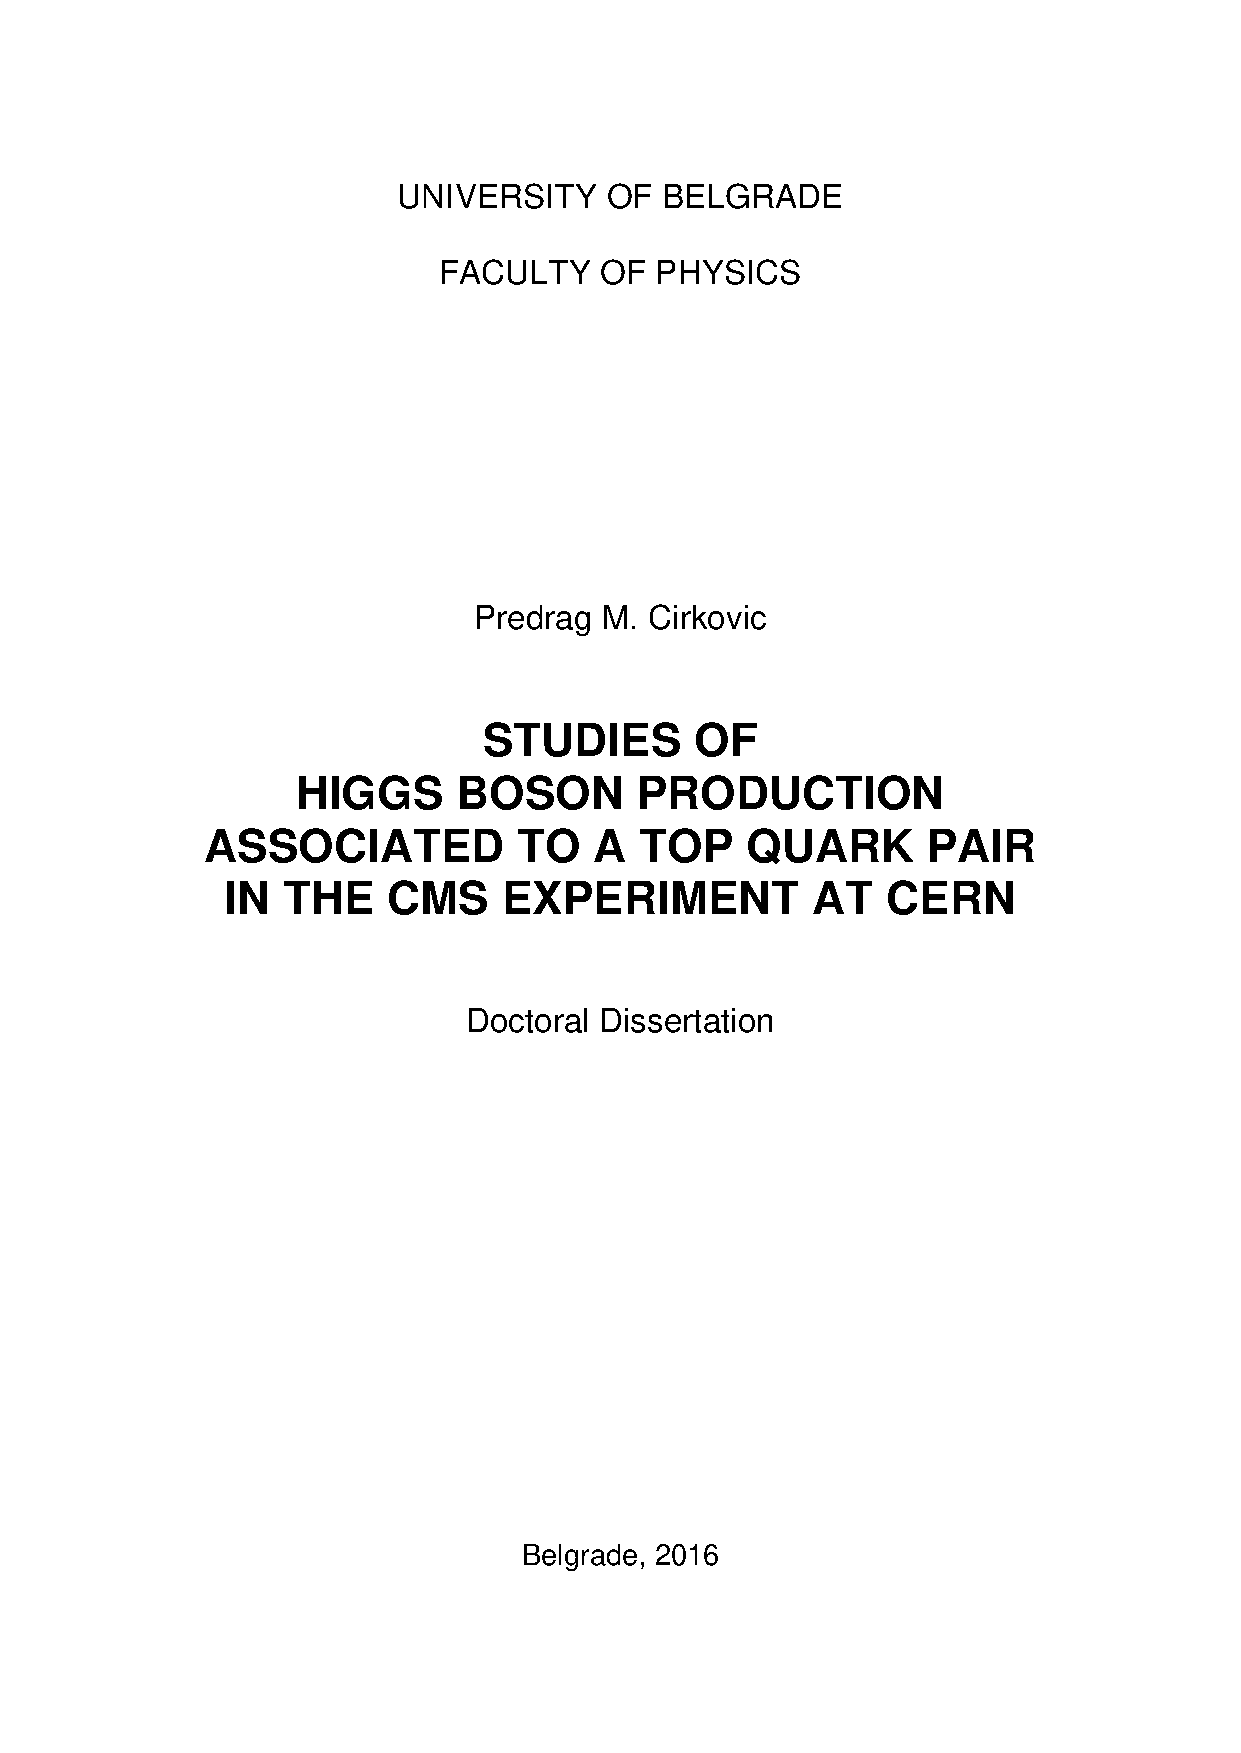
\includepdf[pages=-, pagecommand={\thispagestyle{empty}}, offset=1in -1in]{TitlePages/Title1.pdf}

%%----------------------------------------------------------------------------------------
%%	DECLARATION PAGE
%%	Your institution may give you a different text to place here
%%----------------------------------------------------------------------------------------
%
%\supervisorcommittee{
%
%Supervisor:
%\begin{itemize}
%\item Dr. Miloš Đorđević; Research Fellow / Research Associate (Assistant Research Professor); CERN / University of Belgrade, Vinca Institute of Nuclear Sciences
%\end{itemize}
%Dissertation committee members:
%\begin{itemize}
%\item Prof. Dr. Petar Adžić; Full Professor; University of Belgrade, Faculty of Physics
%\item Dr. Ljiljana Simić; Principal Research Fellow (Full Research Professor); University of Belgrade, Institute of Physics Belgrade
%\item Dr. Jovan Milošević; Senior Research Associate (Associate Research Professor); University of Belgrade, Vinca Institute of Nuclear Sciences
%\end{itemize}
%Date of the dissertation defence: January 1, 2016
%
%}
%\clearpage % Start a new page

%----------------------------------------------------------------------------------------
%	DECLARATION PAGE
%	Your institution may give you a different text to place here
%----------------------------------------------------------------------------------------

\supervisorcommittee{

Ментор:

\begin{itemize}
\item др ...; научни сарадник; Универзитет ..., Институт/Факултет
\end{itemize}
Чланови комисије:
\begin{itemize}
\item проф. др ...; редовни професор; Универзитет ..., Институт/Факултет
\item ...
\end{itemize}

Датум одбране: ...

}
\clearpage % Start a new page

%----------------------------------------------------------------------------------------
%	DECLARATION PAGE
%	Your institution may give you a different text to place here
%----------------------------------------------------------------------------------------

%\Declaration{

%\addtocontents{toc}{\vspace{1em}} % Add a gap in the Contents, for aesthetics

%I, \authornames, declare that this thesis titled, '\ttitle' and the work presented in it are my own. I confirm that:

%\begin{itemize} 
%\item[\tiny{$\blacksquare$}] This work was done wholly or mainly while in candidature for a research degree at this University.
%\item[\tiny{$\blacksquare$}] Where any part of this thesis has previously been submitted for a degree or any other qualification at this University or any other institution, this has been clearly stated.
%\item[\tiny{$\blacksquare$}] Where I have consulted the published work of others, this is always clearly attributed.
%\item[\tiny{$\blacksquare$}] Where I have quoted from the work of others, the source is always given. With the exception of such quotations, this thesis is entirely my own work.
%\item[\tiny{$\blacksquare$}] I have acknowledged all main sources of help.
%\item[\tiny{$\blacksquare$}] Where the thesis is based on work done by myself jointly with others, I have made clear exactly what was done by others and what I have contributed myself.\\
%\end{itemize}
 
%Signed:\\
%\rule[1em]{25em}{0.5pt} % This prints a line for the signature
 
%Date:\\
%\rule[1em]{25em}{0.5pt} % This prints a line to write the date
%}

%\clearpage % Start a new page

%----------------------------------------------------------------------------------------
%	QUOTATION PAGE
%----------------------------------------------------------------------------------------

%\pagestyle{empty} % No headers or footers for the following pages

%\null\vfill % Add some space to move the quote down the page a bit

%\textit{``Thanks to my solid academic training, today I can write hundreds of words on virtually any topic without possessing a shred of information, which is how I got a good job in journalism."}

%\begin{flushright}
%Dave Barry
%\end{flushright}

%\vfill\vfill\vfill\vfill\vfill\vfill\null % Add some space at the bottom to position the quote just right

%\clearpage % Start a new page

%----------------------------------------------------------------------------------------
%	ACKNOWLEDGEMENTS
%----------------------------------------------------------------------------------------

%\setstretch{1.3} % Reset the line-spacing to 1.3 for body text (if it has changed)

\acknowledgements{\addtocontents{toc}{\vspace{1em}} % Add a gap in the Contents, for aesthetics

%Предговор и захвалница иду овде.\ldots
% napisi i predgovor i zahvalnicu…ne znam sta je “predgovor”…uklopi to zajedno u zahvalnicu…jedna do dve strane…moze i samo jedna strana
%Докторска дисертација под називом ''Проучавање продукције Хигџ бозона придруженог пару топ кваркова у експерименту CMS у CERN-у'' представља резултат једне од активности Српске групе CMS у периоду између 2013. и 2016. године.
%
%Рад је изведен у оквиру институција чланица Универзитета у Београду, под покровитељством пројекта ''Физика високих енергија са детектором CMS'' (171019), финансираног од стране Министарства просвете, науке и технолошког развоја.
%Повремени боравци У Европској организацији за нуклеарна истраживања, CERN, ради обављања сервисних активности неопходних за одржавање рада екперименталне апаратуре, финансирани су стране Пројекта за научну сарадњу између земаља источне Европе и Швајцарске (SCOPES).
%
%Захвалност на корисним саветима и несебичној помоћи током рада упућујем пре свега ментору др Милошу Ђорђевићу, затим проф. Петру Аџићу, др Јовану Милошевићу, колегама докторандима Дамиру Деветаку, Милану Стојановићу, као и осталим сарадницима Српске групе CMS, професорима на Физичком факултету, сарадницима у Институту за физику и Институту за нуклеарне науке ''Винча''.
%Такође се захваљујем супрузи Анђи и члановима моје породице на стрпљењу и пруженој подршци.
%
%Захвалница је упућена и члановима CERN-ове радне групе за анализу ttH, као и свим члановима колаборације CMS,
%који су својим преданим радом обезбедили квалитетну организацију рада и функционисање комплетне експерименталне апаратуре и рачунарских ресурса, неопходних за извођење овог истраживања.

Ова докторска дисертација представља резултат једне од активности Српске CMS групе у периоду између 2013. и 2016. године.
...
}
\clearpage % Start a new page

%----------------------------------------------------------------------------------------
%	ABSTRACT PAGE
%----------------------------------------------------------------------------------------

%\addtotoc{Резиме} % Add the "Abstract" page entry to the Contents
\addtotoc{Сажетак} % Add the "Abstract" page entry to the Contents

%\rezime{\addtocontents{toc}{\vspace{1em}} % Add a gap in the Contents, for a esthetics
\rezime{\addtocontents{toc}{\vspace{0em}} % Add to the Contents

\begin{spacing}{1.3}{

У овој дисертацији представљени су резултати истраживања продукције Хигс бозона Стандардног модела (СМ) придруженог пару топ кваркова ($\ttH$).
...

\vfill
Кључне речи: физика високих енергија, ...\\
%Научна област: Експериментална физика честица\\
Научна област: Физика\\
%Ужа научна област: Физика Хигс бозона\\
%Ужа научна област: Физика високих енергија и нуклеарна физика
Ужа научна област: Физика високих енергија и нуклеарна физика
%УДК број:

}\end{spacing}
}

\clearpage % Start a new page

%----------------------------------------------------------------------------------------
%	ABSTRACT PAGE
%----------------------------------------------------------------------------------------

\addtotoc{Abstract} % Add the "Abstract" page entry to the Contents

\abstract{\addtocontents{toc}{\vspace{1em}} % Add a gap in the Contents, for a esthetics
\begin{spacing}{1.3}{

In this dissertation, the search for the production of the Standard Model (SM) Higgs boson associated with the $\ttbar$ pair ($\ttH$) is presented.
...

\vfill
Keywords: high energy physics, ...\\
%Academic Expertise: Experimental particle physics\\
Academic Expertise: Physics\\
%Field of Academic Expertise: Higgs physics\\
%Field of Academic Expertise: High energy physics and nuclear physics
Field of Academic Expertise: High energy physics and nuclear physics
%UDC Number:

}\end{spacing}
}

\clearpage % Start a new page

%----------------------------------------------------------------------------------------
%	LIST OF CONTENTS/FIGURES/TABLES PAGES
%----------------------------------------------------------------------------------------

\pagestyle{fancy} % The page style headers have been "empty" all this time, now use the "fancy" headers as defined before to bring them back

\lhead{\emph{Садржај}} % Set the left side page header to "Contents"
\tableofcontents % Write out the Table of Contents

%\lhead{\emph{List of Figures}} % Set the left side page header to "List of Figures"
%\listoffigures % Write out the List of Figures

%\lhead{\emph{List of Tables}} % Set the left side page header to "List of Tables"
%\listoftables % Write out the List of Tables

%----------------------------------------------------------------------------------------
%	ABBREVIATIONS
%----------------------------------------------------------------------------------------

%\clearpage % Start a new page

%\setstretch{1.5} % Set the line spacing to 1.5, this makes the following tables easier to read

%\lhead{\emph{Abbreviations}} % Set the left side page header to "Abbreviations"
%\listofsymbols{ll} % Include a list of Abbreviations (a table of two columns)
%{
%\textbf{LAH} & \textbf{L}ist \textbf{A}bbreviations \textbf{H}ere \\
%%\textbf{Acronym} & \textbf{W}hat (it) \textbf{S}tands \textbf{F}or \\
%}

%----------------------------------------------------------------------------------------
%	PHYSICAL CONSTANTS/OTHER DEFINITIONS
%----------------------------------------------------------------------------------------

%\clearpage % Start a new page

%\lhead{\emph{Physical Constants}} % Set the left side page header to "Physical Constants"

%\listofconstants{lrcl} % Include a list of Physical Constants (a four column table)
%{
%Speed of Light & $c$ & $=$ & $2.997\ 924\ 58\times10^{8}\ \mbox{ms}^{-\mbox{s}}$ (exact)\\
%% Constant Name & Symbol & = & Constant Value (with units) \\
%}

%%----------------------------------------------------------------------------------------
%%	SYMBOLS
%%----------------------------------------------------------------------------------------
%
%\clearpage % Start a new page
%
%\lhead{\emph{Symbols}} % Set the left side page header to "Symbols"
%
%\listofnomenclature{lll} % Include a list of Symbols (a three column table)
%{
%$a$ & distance & m \\
%$P$ & power & W (Js$^{-1}$) \\
%% Symbol & Name & Unit \\
%
%& & \\ % Gap to separate the Roman symbols from the Greek
%
%$\omega$ & angular frequency & rads$^{-1}$ \\
%% Symbol & Name & Unit \\
%}

%%----------------------------------------------------------------------------------------
%%	DEDICATION
%%----------------------------------------------------------------------------------------
%
%\setstretch{1.3} % Return the line spacing back to 1.3
%
%\pagestyle{empty} % Page style needs to be empty for this page
%
%\dedicatory{For/Dedicated to/To my\ldots} % Dedication text
%
%\addtocontents{toc}{\vspace{2em}} % Add a gap in the Contents, for aesthetics

%----------------------------------------------------------------------------------------
%	THESIS CONTENT - CHAPTERS
%----------------------------------------------------------------------------------------

\mainmatter % Begin numeric (1,2,3...) page numbering

\pagestyle{fancy} % Return the page headers back to the "fancy" style

% Include the chapters of the thesis as separate files from the Chapters folder
% Uncomment the lines as you write the chapters

%\begin{comment}
%% Chapter Template

\chapter{Увод} % Main chapter title

\label{Увод} % Change X to a consecutive number; for referencing this chapter elsewhere, use \ref{ChapterX}

\lhead{Поглавље \thechapter. \emph{Увод}} % Change X to a consecutive number; this is for the header on each page - perhaps a shortened title

Стандардни модел (СМ) представља општеприхваћену физичку теорију која описује све елементарне честице у природи и њихове међусобне интеракције.

...

%\input{OldChapters/StandardModelTheory}
%%\input{OldChapters/HiggsPhysics}
%\input{OldChapters/ExperimentalFacility}
%%\input{OldChapters/LHC}
%%\input{OldChapters/CMSDetector}
%%\input{OldChapters/DataTaking}
%\input{OldChapters/ExperimentalModelDescription}
%%\input{OldChapters/ObjectDefinition}
%%\input{OldChapters/EventSelection}
%%\input{OldChapters/Results&Discussion}
%\input{OldChapters/PhysicsAnalysis}
%% Chapter Template

\chapter{Закључак} % Main chapter title

\label{Закључак} % Change X to a consecutive number; for referencing this chapter elsewhere, use \ref{ChapterX}

\lhead{\emph{Закључак}} % Change X to a consecutive number; this is for the header on each page - perhaps a shortened title

У овој дисертацији представљени су резултати прве потраге за процесом $\ttH$ са детектором CMS на укупној енергији $\sqrt{s}\,=\,13\TeV$ у сударима протона на акцелератору LHC у CERN-у.

...
%\end{comment}

%\begin{comment}
%%% Chapter Template

\chapter{Увод} % Main chapter title

\label{Увод} % Change X to a consecutive number; for referencing this chapter elsewhere, use \ref{ChapterX}

\lhead{Поглавље \thechapter. \emph{Увод}} % Change X to a consecutive number; this is for the header on each page - perhaps a shortened title

Стандардни модел (СМ) представља општеприхваћену физичку теорију која описује све елементарне честице у природи и њихове међусобне интеракције.

...

%%\input{OldChapters/StandardModelTheory}
%%\input{OldChapters/HiggsPhysics}
%%\input{OldChapters/ExperimentalFacility}
%%\input{OldChapters/LHC}
%%\input{OldChapters/CMSDetector}
%%\input{OldChapters/DataTaking}
%%\input{OldChapters/ExperimentalModelDescription}
%%\input{OldChapters/ObjectDefinition}
%%\input{OldChapters/EventSelection}
%%\input{OldChapters/Results&Discussion}
%\input{OldChapters/PhysicsAnalysis}
%%% Chapter Template

\chapter{Закључак} % Main chapter title

\label{Закључак} % Change X to a consecutive number; for referencing this chapter elsewhere, use \ref{ChapterX}

\lhead{\emph{Закључак}} % Change X to a consecutive number; this is for the header on each page - perhaps a shortened title

У овој дисертацији представљени су резултати прве потраге за процесом $\ttH$ са детектором CMS на укупној енергији $\sqrt{s}\,=\,13\TeV$ у сударима протона на акцелератору LHC у CERN-у.

...
%\end{comment}

%%\begin{comment}
%%%\input{Chapters/PreviousResultsAndMotivation}
%% Chapter Template

\chapter{Увод} % Main chapter title

\label{Увод} % Change X to a consecutive number; for referencing this chapter elsewhere, use \ref{ChapterX}

\lhead{Поглавље \thechapter. \emph{Увод}} % Change X to a consecutive number; this is for the header on each page - perhaps a shortened title

Стандардни модел (СМ) представља општеприхваћену физичку теорију која описује све елементарне честице у природи и њихове међусобне интеракције.

...

%% Chapter Template

\chapter{Теоријска поставка} % Main chapter title

\label{Теоријска поставка} % Change X to a consecutive number; for referencing this chapter elsewhere, use \ref{ChapterX}

\lhead{Поглавље \thechapter. \emph{Теоријска поставка}} % Change X to a consecutive number; this is for the header on each page - perhaps a shortened title

...

\section{Хигс бозон у СМ}

\subsection{Хигс потенцијал и нарушење глобалне симетрије}

Хигс поље, илустровано на Сл.~\ref{fig:mexican_hat}, представља скаларни потенцијал у облику ''мексичког шешира''. Описано је једначином~(\ref{eq:V_higgs}) у којој се појављују чланови са имагинарном масом ($\mu^2 < 0$) и $\lambda > 0$.

\begin{equation}
V(\phi) = \mu^2(\phi^*\phi) + \lambda(\phi^*\phi)^2
\label{eq:V_higgs}
\end{equation}

\begin{figure}[H]
  \centering
	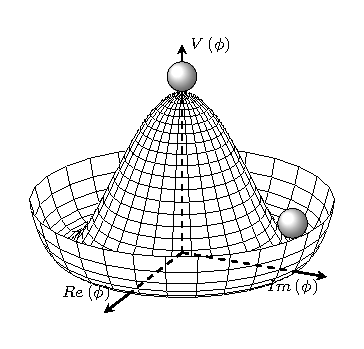
\includegraphics[width=0.505\textwidth]{texImages/mexican_hat.pdf}
	\caption{Облик Хигс потенцијала $V(\phi) = \mu^2(\phi^*\phi) + \lambda(\phi^*\phi)^2$, код којег су $\mu^2 < 0$ и $\lambda > 0$.}
	\label{fig:mexican_hat}
\end{figure}

...

%\input{Chapters/Motivation}
%\input{Chapters/ExperimentalFacility}
%\input{Chapters/PhysicsAnalysis}
%%%\input{Chapters/PhysicsAnalysis8TeV}
%%%\input{Chapters/ResultsDiscussion}
%% Chapter Template

\chapter{Закључак} % Main chapter title

\label{Закључак} % Change X to a consecutive number; for referencing this chapter elsewhere, use \ref{ChapterX}

\lhead{\emph{Закључак}} % Change X to a consecutive number; this is for the header on each page - perhaps a shortened title

У овој дисертацији представљени су резултати прве потраге за процесом $\ttH$ са детектором CMS на укупној енергији $\sqrt{s}\,=\,13\TeV$ у сударима протона на акцелератору LHC у CERN-у.

...
%%\end{comment}

%\begin{comment}
%% Chapter Template

\chapter{Увод} % Main chapter title

\label{Увод} % Change X to a consecutive number; for referencing this chapter elsewhere, use \ref{ChapterX}

\lhead{Поглавље \thechapter. \emph{Увод}} % Change X to a consecutive number; this is for the header on each page - perhaps a shortened title

Стандардни модел (СМ) представља општеприхваћену физичку теорију која описује све елементарне честице у природи и њихове међусобне интеракције.

...

%% Chapter Template

\chapter{Теоријска поставка} % Main chapter title

\label{Теоријска поставка} % Change X to a consecutive number; for referencing this chapter elsewhere, use \ref{ChapterX}

\lhead{Поглавље \thechapter. \emph{Теоријска поставка}} % Change X to a consecutive number; this is for the header on each page - perhaps a shortened title

...

\section{Хигс бозон у СМ}

\subsection{Хигс потенцијал и нарушење глобалне симетрије}

Хигс поље, илустровано на Сл.~\ref{fig:mexican_hat}, представља скаларни потенцијал у облику ''мексичког шешира''. Описано је једначином~(\ref{eq:V_higgs}) у којој се појављују чланови са имагинарном масом ($\mu^2 < 0$) и $\lambda > 0$.

\begin{equation}
V(\phi) = \mu^2(\phi^*\phi) + \lambda(\phi^*\phi)^2
\label{eq:V_higgs}
\end{equation}

\begin{figure}[H]
  \centering
	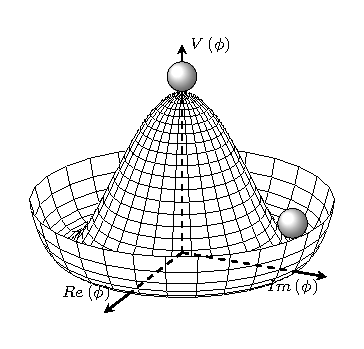
\includegraphics[width=0.505\textwidth]{texImages/mexican_hat.pdf}
	\caption{Облик Хигс потенцијала $V(\phi) = \mu^2(\phi^*\phi) + \lambda(\phi^*\phi)^2$, код којег су $\mu^2 < 0$ и $\lambda > 0$.}
	\label{fig:mexican_hat}
\end{figure}

...

%\input{Chapters/Motivation}
%\input{Chapters/Experiment}
%\input{Chapters/Analysis}
%% Chapter Template

\chapter{Резултати и дискусија} % Main chapter title

\label{Резултати и дискусија} % Change X to a consecutive number; for referencing this chapter elsewhere, use \ref{ChapterX}

\lhead{Поглавље \thechapter. \emph{Резултати и дискусија}} % Change X to a consecutive number; this is for the header on each page - perhaps a shortened title

\section{Резултати}

У овом поглављу дат је кратак преглед коначних резултата анализе продукције $\ttH$ у експерименту CMS, за вредност масе Хигс бозона од $125\GeV$.

...

%% Chapter Template

\chapter{Закључак} % Main chapter title

\label{Закључак} % Change X to a consecutive number; for referencing this chapter elsewhere, use \ref{ChapterX}

\lhead{\emph{Закључак}} % Change X to a consecutive number; this is for the header on each page - perhaps a shortened title

У овој дисертацији представљени су резултати прве потраге за процесом $\ttH$ са детектором CMS на укупној енергији $\sqrt{s}\,=\,13\TeV$ у сударима протона на акцелератору LHC у CERN-у.

...
%\end{comment}

%\begin{comment}
% Chapter Template

\chapter{Увод} % Main chapter title

\label{Увод} % Change X to a consecutive number; for referencing this chapter elsewhere, use \ref{ChapterX}

\lhead{Поглавље \thechapter. \emph{Увод}} % Change X to a consecutive number; this is for the header on each page - perhaps a shortened title

Стандардни модел (СМ) представља општеприхваћену физичку теорију која описује све елементарне честице у природи и њихове међусобне интеракције.

...

% Chapter Template

\chapter{Теоријска поставка} % Main chapter title

\label{Теоријска поставка} % Change X to a consecutive number; for referencing this chapter elsewhere, use \ref{ChapterX}

\lhead{Поглавље \thechapter. \emph{Теоријска поставка}} % Change X to a consecutive number; this is for the header on each page - perhaps a shortened title

...

\section{Хигс бозон у СМ}

\subsection{Хигс потенцијал и нарушење глобалне симетрије}

Хигс поље, илустровано на Сл.~\ref{fig:mexican_hat}, представља скаларни потенцијал у облику ''мексичког шешира''. Описано је једначином~(\ref{eq:V_higgs}) у којој се појављују чланови са имагинарном масом ($\mu^2 < 0$) и $\lambda > 0$.

\begin{equation}
V(\phi) = \mu^2(\phi^*\phi) + \lambda(\phi^*\phi)^2
\label{eq:V_higgs}
\end{equation}

\begin{figure}[H]
  \centering
	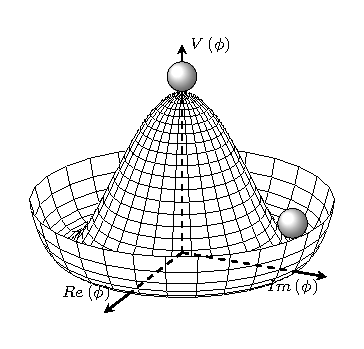
\includegraphics[width=0.505\textwidth]{texImages/mexican_hat.pdf}
	\caption{Облик Хигс потенцијала $V(\phi) = \mu^2(\phi^*\phi) + \lambda(\phi^*\phi)^2$, код којег су $\mu^2 < 0$ и $\lambda > 0$.}
	\label{fig:mexican_hat}
\end{figure}

...

% Chapter Template

\chapter{Разрада} % Main chapter title

\label{Разрада} % Change X to a consecutive number; for referencing this chapter elsewhere, use \ref{ChapterX}

\lhead{Поглавље \thechapter. \emph{Разрада}} % Change X to a consecutive number; this is for the header on each page - perhaps a shortened title

\section{Досадашњи резултати потрага за Хигс бозоном}

У циљу изучавања физике СМ претходних деценија предлагани су и коришћени су различити експерименти и акцелераторске машине.

...

Регистровани сигнал, мерен у односу на референтни ниво фона, најизраженији у каналима распада $H\rightarrow\gamma\gamma$ и $H\rightarrow ZZ\rightarrow 4l$, одређен је са укупним статистичким значајем од $5\sigma$. То је показано на Сл.~\ref{fig:p-value_CMS}~\cite{Chatrchyan:2013lba}, на којој је дато поређење дијаграма зависности $p$-вредности за различите канале распада Хигс бозона ($H \rightarrow \gamma\gamma$, $ZZ$, $WW$, $\tau\tau$ и $bb$), као и дијаграм који одговара комбинацији тих канала (\textit{Combined obs.}).

\begin{figure}[H]
  \centering
	\includegraphics[width=0.705\textwidth]{Figs/figures_comb_sqr_pvala_all_bydecay_smallGGScale_wideX.eps}
	\caption{p-вредност у зависности од масе Хигс бозона добијена анализом експерименталних података са експеримента CMS~\cite{Chatrchyan:2013lba}.
	p-вредност је мера статистичког значаја добијена тестирањем одређене хипотезе, чија вредност одговара вероватноћи да одређени догађај не представља последицу статистичких флуктуација.}
	\label{fig:p-value_CMS}
\end{figure}

...

%\section{Резултати претходних потрага и мотивација за проучавање процеса ttH}
\section{Мотивација за проучавање процеса ttH}

...

У Таб.~\ref{tab:channelSummary} дат је преглед коначних стања и одговарајућих услова селекције физичких објеката за сваку од анализа $\ttH$ на енергији $\sqrt{s}\,=\,8\TeV$.

\begin{table}[H]
\begin{center}
\small
\caption{
Преглед канала, коначних стања и основних услова селекције коришћених у анализи $\ttH$.
У првој колони, канали распада Хигс бозона класификовани су према типу распада (хадронски, фотонски или лептонски);
у другој колони, коначна стања описана симболички тако да $l$ представља лептон (електрон или мион), $\gamma$ - фотон, $j$ - џет, $b$ - џет идентификован да је настао из b кварка, $\tau_h$ - џет настао хадронским распадом $\tau$ лептона.
У трећој колони су приказани одговарајући тригери коришћени за преселекцију догађаја,
а у четвртој колони дат је преглед основних услова селекције реконструисаних физичких објеката~\cite{Khachatryan:2014qaa}.
}
\label{tab:channelSummary}
\resizebox{1.0\linewidth}{!}{
\begin{tabular}{|l|l|l|l|} \hline
Category                     & Signature          & Trigger       & Signature \\ \hline \hline
& Lepton + Jets      & Single Lepton & 1\ $ e $/$ \mu $, $ p_T  > 30 \GeV$ \\
{\bf \boldmath$ H  \rightarrow $ Hadrons} & ($\ttbar  H  \rightarrow   l    \nu \mathrm{jj}  b  b  b   b $)& & $\geq 4$\ jets + $\geq 2$\ b-tags, $ p_T  > 30 \GeV$ \\
\cline{2-4}
\ \ \ $ H  \rightarrow   bb $ & Dilepton  & Dilepton      & 1\ $ e $/$ \mu $, $ p_T  > 20 \GeV$  \\
\ \ \ $ H  \rightarrow   \tau _\mathrm{h} \tau _\mathrm{h}$ & ($\ttbar  H  \rightarrow   l    \nu  l    \nu  b  b  b   b $) & & 1\ $ e $/$ \mu $, $ p_T  > 10 \GeV$  \\
\ \ \ $ H  \rightarrow   W   W $            &                    &               & $\geq 3$\ jets + $\geq 2$\ b-tags, $ p_T  > 30 \GeV$ \\
\cline{2-4}
& Hadronic $ \tau $    & Single Lepton & 1 $ e $/$ \mu $, $ p_T  > 30\GeV$ \\
& ($\ttbar  H  \rightarrow   l    \nu  \tau _\mathrm{h} [  \nu]  \tau _\mathrm{h} [  \nu] \mathrm{jj}  b  b $) & & 2\ $ \tau _\mathrm{h}$, $ p_T  > 20 \GeV$ \\
&                    &               & $\geq\ 2$\ jets + 1-2\ b-tags, $ p_T  > 30 \GeV$ \\
\hline
& Leptonic           & Diphoton      & 2\ $ \gamma $, $ p_T  > m_{ \gamma  \gamma }/2\,(25) \GeV$ for 1$^{\mathrm{st}}$ (2$^{\mathrm{nd}}$) \\
{\bf \boldmath$ H  \rightarrow  $ Photons} & ($\ttbar  H  \rightarrow   l    \nu \mathrm{jj}  b  b  \gamma   \gamma $, & & $\geq 1$\ $ e $/$ \mu $, $ p_T  > 20 \GeV$ \\
\ \ \ $ H  \rightarrow   \gamma   \gamma $       &  $\ttbar  H  \rightarrow   l    \nu  l    \nu  b  b   \gamma   \gamma $)& & $\geq 2$\ jets + $\geq 1$\ b-tags, $ p_T  > 25 \GeV$ \\
\cline{2-4}
& Hadronic           & Diphoton      & 2\ $ \gamma $, $ p_T  > m_{ \gamma  \gamma }/2\,(25) \GeV$ for 1$^{\mathrm{st}}$ (2$^{\mathrm{nd}}$) \\
& ($\ttbar  H  \rightarrow  \mathrm{jj} \mathrm{jj}  b  b  \gamma   \gamma $)& & 0\ $ e $/$ \mu $, $ p_T  > 20 \GeV$ \\
&                    &               & $\geq 4$\ jets + $\geq 1$\ b-tags, $ p_T  > 25 \GeV$ \\
\hline
& Same-Sign Dilepton & Dilepton      & 2\ $ e $/$ \mu $, $ p_T  > 20 \GeV$  \\
{\bf \boldmath $ H  \rightarrow  $ Leptons} & ($\ttbar  H  \rightarrow   l ^\pm   \nu  l ^\pm [  \nu] \mathrm{jjj[j]}  b  b $) & & $\geq 4$\ jets + $\geq 1$\ b-tags, $ p_T  > 25 \GeV$ \\
\cline{2-4}
\ \ \ $ H  \rightarrow   W  W $          & 3 Lepton           & Dilepton,     & 1\ $ e $/$ \mu $, $ p_T  > 20 \GeV$  \\
\ \ \ $ H  \rightarrow   \tau  \tau $        & ($\ttbar  H  \rightarrow   l    \nu  l  [  \nu]  l  [  \nu] \mathrm{j[j]}  b  b $)&  Trielectron & 1\ $ e $/$ \mu $, $ p_T  > 10 \GeV$  \\
\ \ \ $ H  \rightarrow   Z  Z $        &                    &               & 1\ $ e $($ \mu $), $ p_T  > 7(5) \GeV$  \\
&                    &               & $\geq 2$\ jets + $\geq 1$\ b-tags, $ p_T  > 25 \GeV$ \\
\cline{2-4}
& 4 Lepton           & Dilepton,     & 1\ $ e $/$ \mu $, $ p_T  > 20 \GeV$  \\
& ($\ttbar  H  \rightarrow   l    \nu  l    \nu  l  [  \nu]  l  [  \nu]  b  b $) &  Trielectron & 1\ $ e $/$ \mu $, $ p_T  > 10 \GeV$  \\
&                    &               & 2\ $ e $($ \mu $), $ p_T  > 7(5) \GeV$  \\
&                    &               & $\geq 2$\ jets + $\geq 1$\ b-tags, $ p_T  > 25 \GeV$ \\
\hline
\end{tabular}
}
\end{center}
\end{table}

%\input{Chapters/Motivation}
%\input{Chapters/Experiment}
%\input{Chapters/Analysis}
% Chapter Template

\chapter{Резултати и дискусија} % Main chapter title

\label{Резултати и дискусија} % Change X to a consecutive number; for referencing this chapter elsewhere, use \ref{ChapterX}

\lhead{Поглавље \thechapter. \emph{Резултати и дискусија}} % Change X to a consecutive number; this is for the header on each page - perhaps a shortened title

\section{Резултати}

У овом поглављу дат је кратак преглед коначних резултата анализе продукције $\ttH$ у експерименту CMS, за вредност масе Хигс бозона од $125\GeV$.

...

%\input{Chapters/Update}
% Chapter Template

\chapter{Закључак} % Main chapter title

\label{Закључак} % Change X to a consecutive number; for referencing this chapter elsewhere, use \ref{ChapterX}

\lhead{\emph{Закључак}} % Change X to a consecutive number; this is for the header on each page - perhaps a shortened title

У овој дисертацији представљени су резултати прве потраге за процесом $\ttH$ са детектором CMS на укупној енергији $\sqrt{s}\,=\,13\TeV$ у сударима протона на акцелератору LHC у CERN-у.

...
%\end{comment}

%----------------------------------------------------------------------------------------
%	THESIS CONTENT - APPENDICES
%----------------------------------------------------------------------------------------

\addtocontents{toc}{\vspace{2em}} % Add a gap in the Contents, for aesthetics

\appendix % Cue to tell LaTeX that the following 'chapters' are Appendices
\renewcommand{\thechapter}{\Roman{chapter}}

%\appendixpage
%\begin{appendices}
%\input{Appendices/AppendixA}
%\input{Appendices/AppendixB}
%\end{appendices}

% Include the appendices of the thesis as separate files from the Appendices folder
% Uncomment the lines as you write the Appendices

%\begin{comment}
% Appendix A

\chapter{Наслов додатка} % Main appendix title

\label{ДодатакI} % For referencing this appendix elsewhere, use \ref{AppendixA}

\lhead{Додатак I \emph{Наслов додатка}} % This is for the header on each page - perhaps a shortened title

Текст додатка.
% Appendix B

\chapter{Наслов додатка} % Main appendix title

\label{ДодатакII} % For referencing this appendix elsewhere, use \ref{AppendixA}

\lhead{Додатак II \emph{Наслов додатка}} % This is for the header on each page - perhaps a shortened title

Текст додатка.
%\end{comment}
%\input{Appendices/AppendixC}

\addtocontents{toc}{\vspace{2em}} % Add a gap in the Contents, for aesthetics

\backmatter

%----------------------------------------------------------------------------------------
%	BIBLIOGRAPHY
%----------------------------------------------------------------------------------------

\label{Литература}

\addtotoc{Литература}

\lhead{\emph{Литература}} % Change the page header to say "Bibliography"

%\bibliographystyle{unsrtnat} % Use the "unsrtnat" BibTeX style for formatting the Bibliography

\printbibliography

%\xpatchbibmacro{date+extrayear}{%
  %\printtext[parens]%
%}{%
  %\setunit{\addperiod\space}%
  %\printtext%
%}{}{}
%
%\printbibliography

%\patchbibmacro{date+extrayear}{%
  %\printtext[parens]%
%}{%
  %\setunit{\addperiod\space}%
  %\printtext%
%}{}{}
%
%\printbibliography

%----------------------------------------------------------------------------------------
%	BIOGRAPHY
%----------------------------------------------------------------------------------------

%\input{Appendices/Biography}

\clearpage % Start a new page

%----------------------------------------------------------------------------------------
%	BIBLOOGRAPHY
%----------------------------------------------------------------------------------------

%\input{Appendices/Bibliography}

\clearpage % Start a new page

%----------------------------------------------------------------------------------------
%	DECLARATION PAGE
%	Your institution may give you a different text to place here
%----------------------------------------------------------------------------------------

%\Declaration{
%\begin{figure}[t!]
	%\includegraphics[width=\pagewidth]{Figures/Declarations/Declaration1.pdf}
%\end{figure}
%}

%\includepdf[pages=-, pagecommand={\thispagestyle{empty}}, offset=1in -1in]{Declarations/Declaration1Filled.pdf}
%\includepdf[pages=-, pagecommand={\thispagestyle{empty}}, offset=1in -1in]{Declarations/Declaration2Filled.pdf}
%\includepdf[pages=-, pagecommand={\thispagestyle{empty}}, offset=1in -1in]{Declarations/Declaration3Filled.pdf}

%\includepdf[pages=-, pagecommand={\thispagestyle{empty}}, offset=1in -1in]{Declarations/DeclarationsFilled.pdf}

%\Declaration{
%
%\addtocontents{toc}{\vspace{1em}} % Add a gap in the Contents, for aesthetics
%
%\setstretch{0}
%\fontsize{12pt}{0}\selectfont
%\vspace{36pt}
%{\bf Прилог 1.\par}
%\vspace{10pt}
%\centering
%\vspace{12pt}
%\fontsize{16pt}{0}\selectfont
%{\bf Изјава о ауторству \par}
%\vspace{3pt}
%\fontsize{11pt}{0}\selectfont
%{\bf \par}\vspace{10pt}
%{\bf \par}\vspace{10pt}
%{\bf \par}\vspace{10pt}
%\raggedright
%{Потписани-a \par}
%\vspace{10pt}
%{број индекса \par}
%\vspace{10pt}
%{\bf \par}\vspace{10pt}
%\centering
%{\bf Изјављујем \par}
%\vspace{10pt}
%\raggedright
%{да је докторска дисертација под насловом \par}
%\vspace{10pt}
%\setstretch{1.3}
%\begin{itemize}
%\item резултат сопственог истраживачког рада,
%\item да предложена дисертација у целини ни у деловима није била предложена за добијање било које дипломе према студијским програмима других високошколских установа,
%\item да су резултати коректно наведени и
%\item да нисам кршио/ла ауторска права и користио интелектуалну својину других лица.
%\end{itemize}
%\setstretch{0}
%\raggedleft
%{\bf Потпис докторанда \par}
%\vspace{10pt}
%\raggedright
%{У Београду, \par}
%\vspace{10pt}
%\vfill
%
%}

%----------------------------------------------------------------------------------------
%	DECLARATION PAGE
%	Your institution may give you a different text to place here
%----------------------------------------------------------------------------------------

%\Declaration{
%
%\addtocontents{toc}{\vspace{1em}} % Add a gap in the Contents, for aesthetics
%
%\setstretch{0}
%\fontsize{12pt}{0}\selectfont
%{ \par}
%\fontsize{11pt}{10}\selectfont
%{\bf Прилог 2.\par}
%{ \par}
%\vspace{12pt}
%\fontsize{16pt}{10}\selectfont
%Изјава o истоветности штампане и електронске верзије докторског рада
%\vspace{3pt}
%\vfill
%
%}

%----------------------------------------------------------------------------------------

\end{document}  